\documentclass[12pt,letterpaper]{article}
\usepackage[utf8]{inputenc}
\usepackage{amsmath,amssymb,fullpage,graphicx}
\usepackage{subfigure}
\usepackage{amssymb}

\begin{document}

\subsection*{Q4-a}

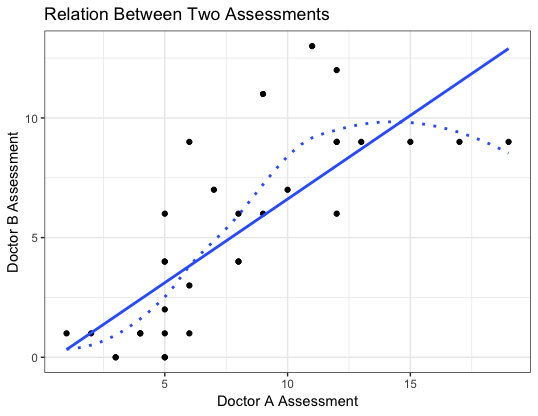
\includegraphics[width=150mm]{hw2-q4.png}

\begin{verbatim}
> cor(assessment_data$DoctorA, assessment_data$DoctorB)
[1] 0.7751628
\end{verbatim}

\noindent The correlation coefficient between assessments of two doctors is 0.77,  which indicates they are somehow positive related. \\

\noindent Their positive correlation can also be perceived from the scatter plot. However, I don't think the relationship is linear. The blue line is the linear curve between these two variables, and we can perceive this curve doesn't fit the data very well, i.e. the residual turns out to be larger as x, y values rise up. 

\subsection*{Q4-b}

\noindent We assumed that the data from two assessments are both normally distributed, and the observations are independent to each other.\\

\noindent A paired sample t-test can be applied on sample data to figure out whether there is a difference between two doctor's assessments.  \\

\noindent In this test, $H_0$ assumes the mean difference between two sets of data (paired sample) is zero. \\

\noindent $H_1$ states the mean difference is non-zero (two-sided test)\\

\noindent First calculate the mean difference $\bar{d}$ and standard error $SE(\bar{d}) = \frac{Sd(d)}{\sqrt[]{n}}$, where $n = 32$, the sample size. \\

\noindent Then calculate the t-statistic $T = \frac{\bar{d} - \mathbb{E}(\bar{d})}{SE(\bar{d})} = \frac{\bar{d}}{SE(\bar{d})}$. Under the null, t-statistic should follow a t-distribution with degree of freedom $(n - 1) = 31$. \\

\noindent Use the t-statistic to find its p-value for two-tails on t-distribution with $df = 31$, and compare the p-value to size of the test $\alpha$. Reject the null if p-value $\leq \alpha$.

\subsection*{Q4-c}
\begin{verbatim}
> t.test(arc_data$DoctorA, arc_data$DoctorB, alternative = 'two.sided', paired = T)

	Paired t-test

data:  arc_data$DoctorA and arc_data$DoctorB
t = 5.5, df = 31, p-value = 5.12e-06
alternative hypothesis: true difference in means is not equal to 0
95 percent confidence interval:
 1.730243 3.769757
sample estimates:
mean of the differences 
                   2.75 
\end{verbatim}

\noindent We may perceive from the summary of this paired t-test that p-value has an extremely small value $5.12 \times 10^{-6}$. Under the test size 0.05, p-value $\leq \alpha = 0.05$, so it's significant to reject the null hypothesis that mean difference is zero. Also, the test summary shows the confidence interval based on sample mean difference is 1.73 to 3.77, excluded from 0. 


\subsection*{Q4-d}
\noindent If a test result shows a p-value $> \alpha$, it's not necessarily to mean that this type of assessment is highly reproducible. We may interpret the test result as failing to reject the null hypothesis. Fail to reject is different from accepting the null, because one of the reasons we fail to reject the null is the low power of the test. 

\end{document}